\chapter{Coherent Light and Single Photons}
\label{sec:5_coherent_light_single_photons}

In this Lesson, we will look at why light is such an integral part of modern day communication.
We will discuss the difference between coherent and incoherent light, and outline the basic principle behind producing coherent light using lasers.
Finally, we will transition to talking about light in the context of quantum communication that relies on single photons as information carriers.

\section{Introduction}
\label{sec:5-1_intoduction}

Why do we want to encode information as optical signals?
Light is a very good carrier of information because it is incredibly \textit{\textbf{fast}}.
Table~\ref{tab:5-1_speed_light} summarizes the speed of light in various media.
\begin{table}[b!]
    \centering
    \begin{tabular}{c|c|c}
        vacuum & $c$ & $2.998\times10^{8} \; \text{ms}^{-1}$  \\
        \hline
        air & $c/1.0003$ & $2.998\times10^{8} \; \text{ms}^{-1}$  \\
        \hline
        silica fiber & $c/1.47$ & $2.039\times10^{8} \; \text{ms}^{-1}$
    \end{tabular}
    \caption[Speed of light]{Speed of light in various media.}
    \label{tab:5-1_speed_light}
\end{table}
In vacuum, the speed of light by $c=2.998\times 10^8$ $\text{ms}^{-1}$.
We do not send light through vacuum most of the time.
However, even in air the light slows by only a factor of 1.0003.
Most often, we use fiber optic cables made from pure silica glass with refractive index of 1.47.
This decreases the speed of light somewhat but still remains very fast.

Apart from being fast, light is also relatively \textit{\textbf{easy to produce}}.
Even in the early days, a reliable source of light was fire.
We saw an example of this when we learnt about optical telegraphy used for rapid communication on the Great Wall of China in Lesson~\ref{sec:1_Introduction}.
Today, we mainly use lasers and send the optical signals through fibers.
Due to their ability to produce highly coherent light, lasers had a transformative impact not only on the way we communicate but on many other aspects of our lives. 

The third reason why light is so useful in communication is that photons do not interact easily with each other.
Once in flight, photons will continue speeding to their destination nearly unaffected.
This makes optical signals \textit{\textbf{robust to noise}}.
Compare this with copper wires carrying electric signals.
The moving electrons are susceptible to external electric and magnetic noise and require thorough shielding to protect the integrity of the signal.
Furthermore, the moving electrons themselves produce electromagnetic fields which may affect other nearby carriers of electric signals.
This means that copper wires cannot be packed too closely to each other.
In contrast, this is not the case for optical fibers.

\begin{figure}[t]
    \centering
    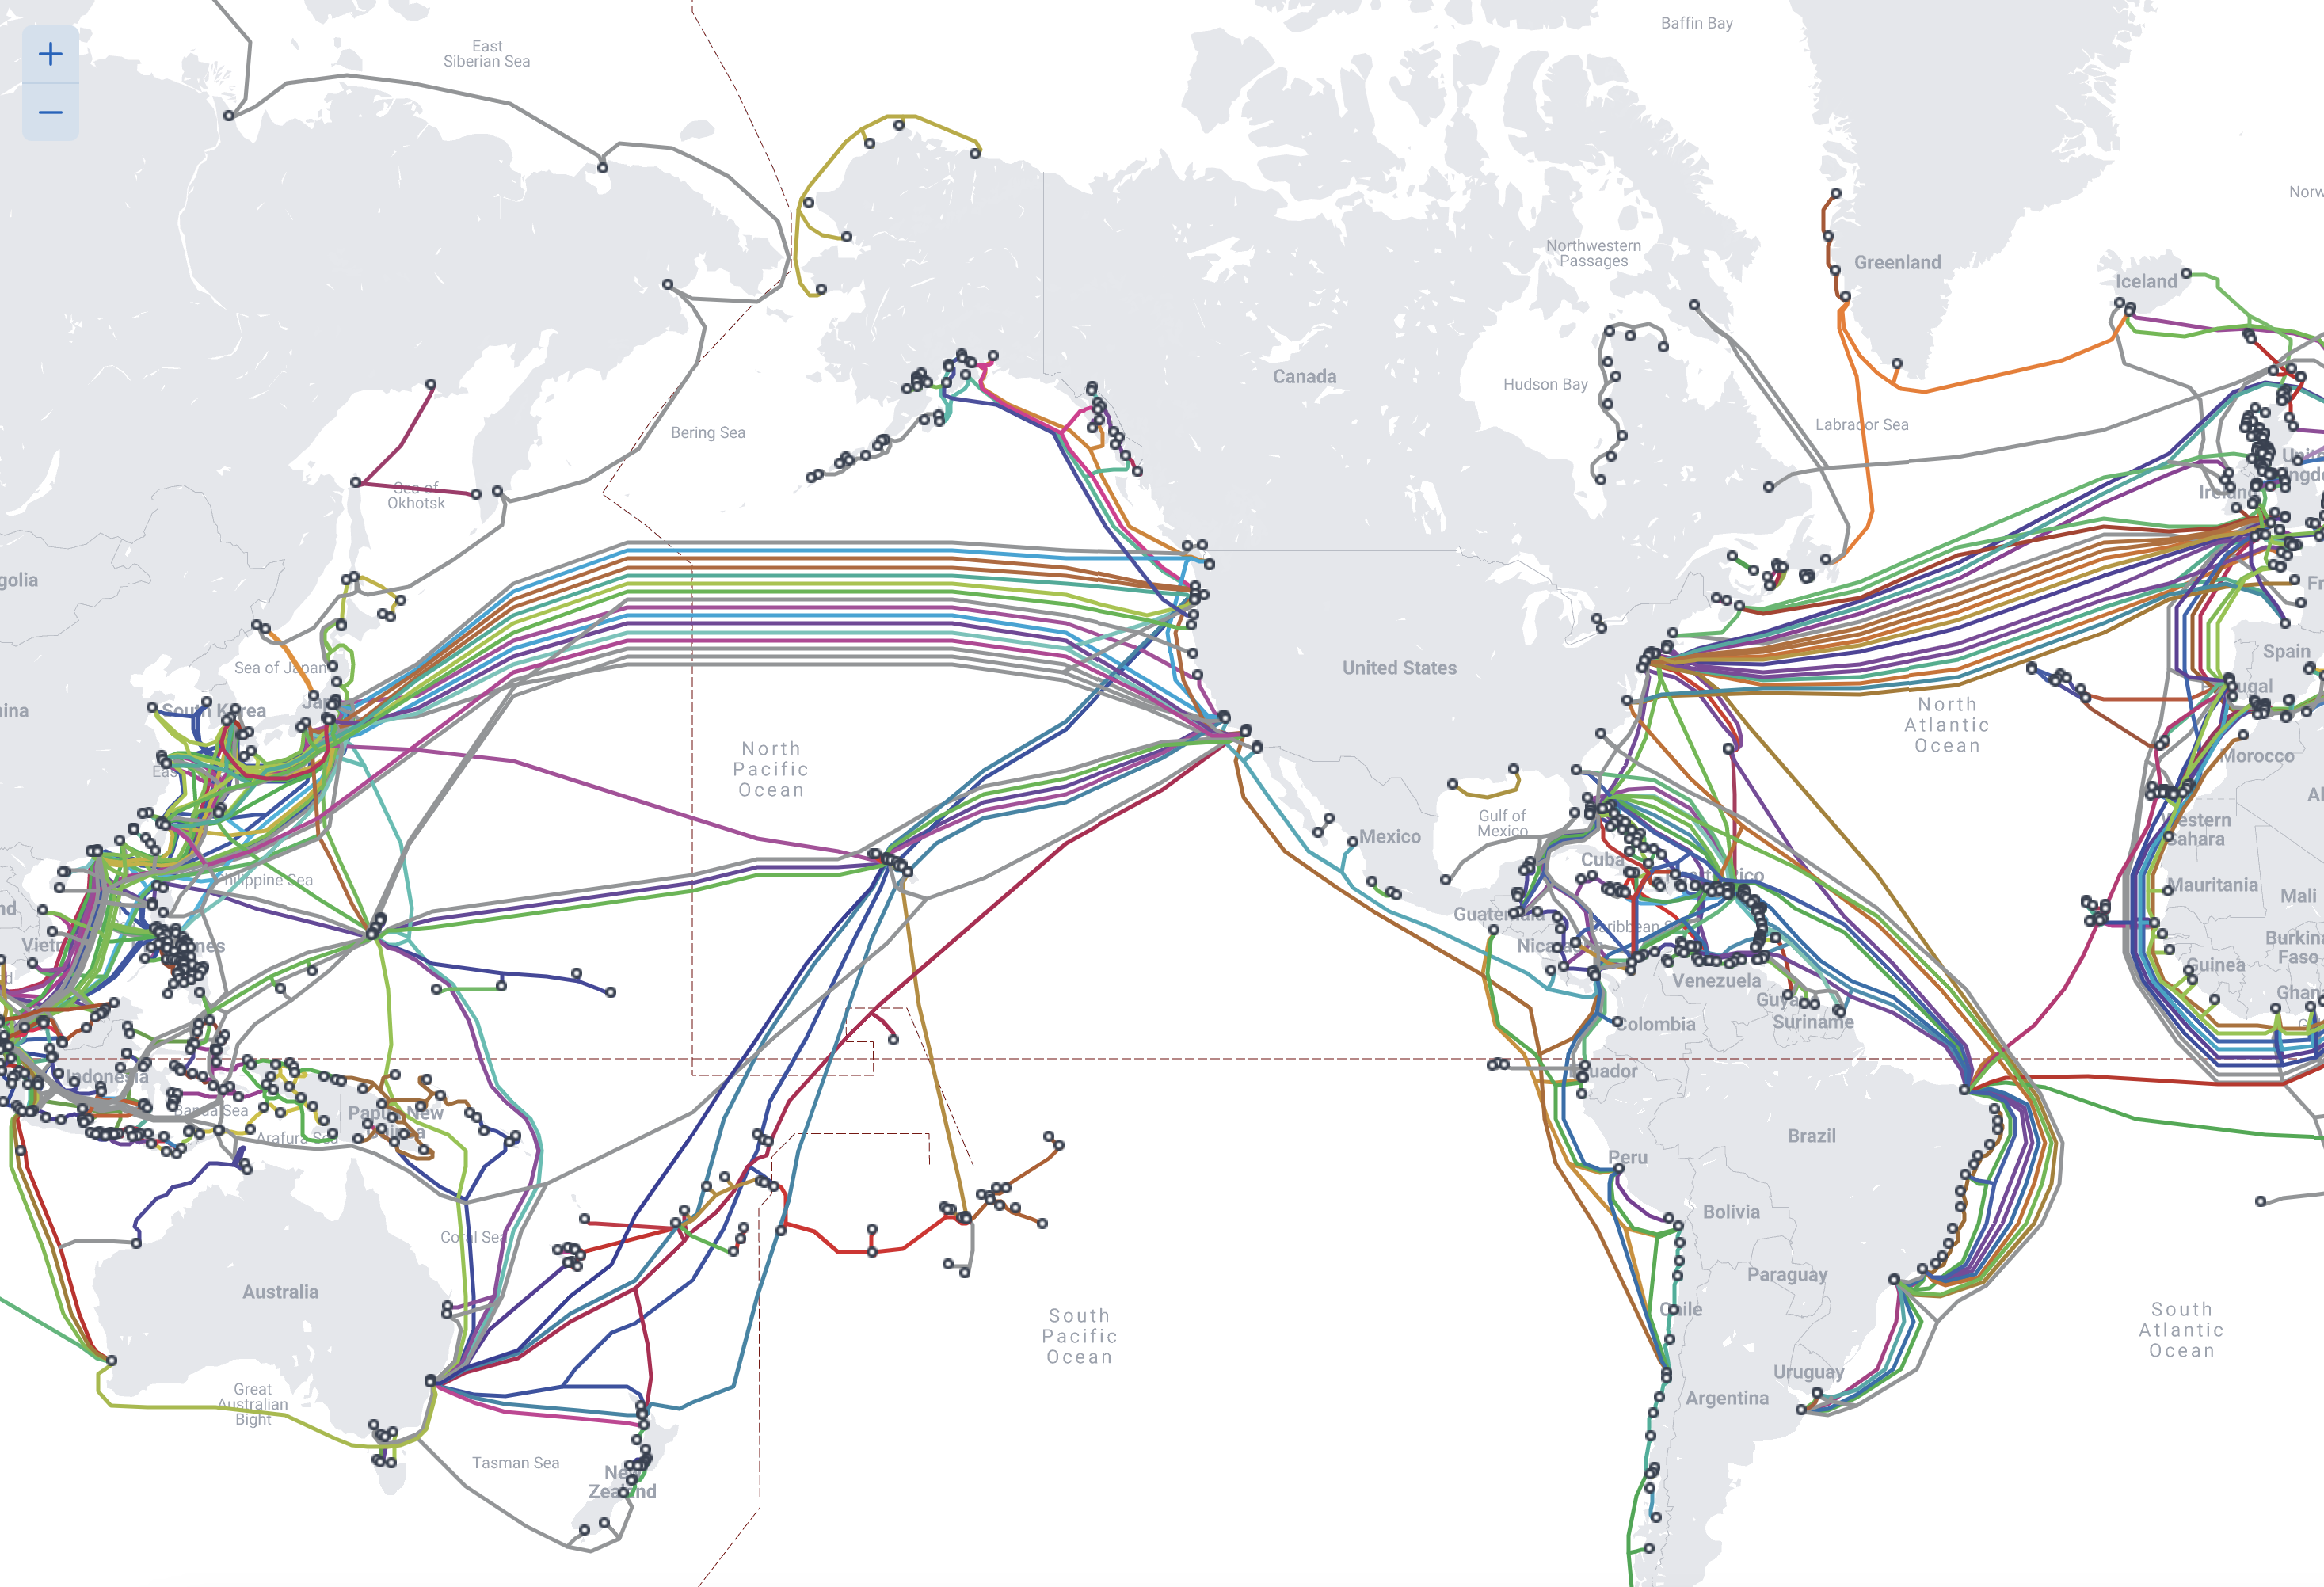
\includegraphics[width=0.8\textwidth]{lesson5/5-1_underwater_cable_map.png}
    \caption[Underwater cabel map]{Map of submarine cables.}
    \label{fig:5-1_underwater_cable_map}
\end{figure}

Optics has always played an important role in communication.
We saw a couple of examples of that already in the Great Wall of China and Napoleon's semaphore in Lesson~\ref{sec:1_Introduction}.
These methods were limited in the sense that you had to have a direct visual path between the sender and the receiver, you needed good weather conditions, and in the case of Napoleon's semaphore, it only worked during the day.
\textit{\textbf{Waveguides}} circumvent all these problems.
Use of electric wires and optical fibers sparked a rapid expansion in our ability to communicate fast and far.
Figure~\ref{fig:5-1_underwater_cable_map} shows a map of submarine cables \footnote{This map was obtained from TeleGeography at \href{https://www.submarinecablemap.com/}{https://www.submarinecablemap.com/} under the \href{https://creativecommons.org/licenses/by-sa/4.0/}{CC BY-SA 4.0} license.}, connecting the continents.
It is these cables that allow seamless global communication at incredible speeds.

In this lesson, we are going to be concerned with how to produce three types of light.
We will begin with \textit{\textbf{incoherent light}}.
This is light that can be produced by burning fuel or heating a gas.
We will explain in what sense is this light incoherent and what it means in Section~\ref{sec:5-2_coherent_vs_incoherent}.
Incoherent light is very easy to produce, which is why it played an important historical role as we have discussed already.
This type of light is known as a classical state of light as it does not manifest any quantum behavior.

We will compare incoherent light with \textit{\textbf{coherent light}} produced by lasers. The main mechanism behind producing this light is known as stimulated emission, which we will discuss in Sec.~\ref{sec:5-3_lasers1} and Sec.~\ref{sec:5-4_lasers2}.
Lasers sparked the first information revolution and therefore play an important historical role.
Despite its coherent nature, light produced by lasers is still not fully quantum. 
Developments in laser technology over the last decades have led to great proliferation of available sources of coherent light.
Lasers range from large and powerful ones found in high-tech laboratories to small pointer devices hanging from our keychains.

We will conclude this lesson by looking at \textit{\textbf{single photon sources}} in Sec~\ref{sec:5-5_single_photons}.
We will discuss three ways of producing single photons.
The first one is by attenuation of laser light.
the second method is by using heralded photons.
The third way is to use genuine emitters of single photons, such as nitrogen vacancy centres in diamond.
Compared to the previous two types of light, single photons are very difficult to make.
They can be only produced under very stringent requirements in laboratories, but they can display quantum behavior which is why they are crucial in quantum communication.


\section{Coherent vs incoherent light}
\label{sec:5-2_coherent_vs_incoherent}

\begin{figure}
    \centering
    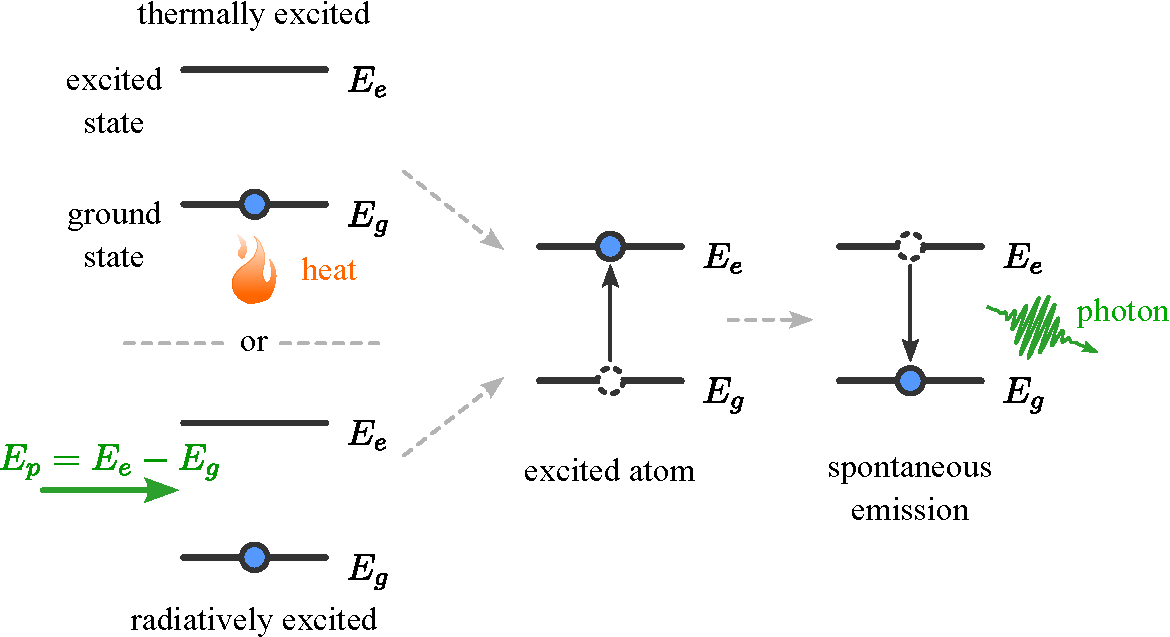
\includegraphics[width=\textwidth]{lesson5/5-2_spontaneous_emission.pdf}
    \caption[Spontaneous emission]{A two-level atom is excited either thermally or radiatively. After some time it deexcites via spontaneous emission producing a photon of light.}
    \label{fig:5-2_spontaneous_emission}
\end{figure}

How does matter radiate light?
Let's consider a model of a simple two-level atom as shown in Fig.~\ref{fig:5-2_spontaneous_emission}.
The ground state has energy $E_g$ and the excited state has energy $E_e$.
The state in of the atom is pictured by the blue circle.
In order to produce light, the atom needs to first receive energy.
One way to do that is through het.
If this is the case, we say the atom becomes \textit{\textbf{thermally excited}}.
Another way is to excite the atom with radiation.
A different way of exciting the atom is to irradiate it with light of the right energy.
The atom can absorb radiation of energy equal to the difference of energies between the excited and ground states, $E_p = E_e - E_g$.
When this happens, we say the atoms has be \textit{\textbf{radiatively excited}}.
After some time, the atom releases the stored energy in the form of a photon of light.
This process happens without an external stimulus at a random time and is called \textit{\textbf{spontaneous emission}}.

Let's consider two such excited atoms as shown in Fig.~\ref{fig:5-2_incoherent_emission}.
After some time, both atoms undergo the process of spontaneous emission producing one photon each.
The direction of emission is random and therefore different for both atoms.
Furthermore, both photons have random and different phases.
We call such light to be incoherent.

We can go one step further and consider a large amount of atoms emitting light.
To be more specific, we can consider an incandescent light bulb.
Here, a filament is heated up by an electric current running through it.
This in turn excites the atoms in the filament which eventually undergo spontaneous emission producing a large amount of photons.
Not only are these photons travelling in all possible directions and are out to phase, their energies are different as well.
This is because the atoms in the filament have much more complicated energy level structure than our simple two-level model.
In conclusion, incoherent light is composed of components with different energies travelling in different directions, each having a different phase.

\begin{figure}
    \centering
    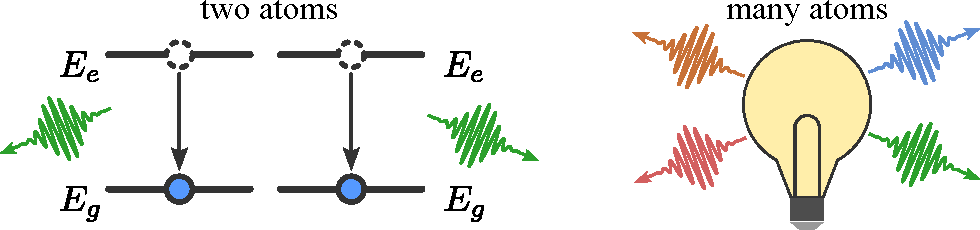
\includegraphics[width=0.8\textwidth]{lesson5/5-2_incoherent_emission.pdf}
    \caption[Incoherent emission]{Caption}
    \label{fig:5-2_incoherent_emission}
\end{figure}

The question that you might be asking yourself is what does it take to produce light the opposite is true.
How can we make light where it has a single component of the same energy, travelling in the same direction and is of the same phase?
We will answer this question in the next two sections.



\section{Lasers I: Stimulated emission}
\label{sec:5-3_lasers1}

%Step three: lasers, one.

In this step, we address the question that was raised at the end of the previous step.
What are the basic ingredients to make coherent light.
Such light is in-phase, monochromatic and travels in the same direction.
Typical example of a source that produces light with these properties is the \textit{\textbf{laser}}.
Laser stands for ``light amplification via stimulated emission of radiation''.
Let's have a look at what these individual words mean.

We begin with \textit{\textbf{stimulated emission}}, which is the physical process behind lasing.
We have encountered two of the three fundamental ways in which light interacts with matter, namely stimulated absorption and spontaneous emission, also shown in Fig.~\ref{fig:5-3_light_matter_interaction}.
Stimulated absorption is when an atom, initially in the ground state interacts with an incoming photon. If the frequency of the photon is just right, the atom may absorb this photon, and the atom becomes excited.
Spontaneous emission is when an initially excited atom emits a photon of light without any external stimulus.
Stimulated emission on the other hand is when an initially excited atom interacts with an incoming photon.
This causes the atom to emit a photon of light.
But this time, the emitted photon of light has the same energy as the external photon, same phase and crucially it is emitted in the same direction.
In other words, the two photons are coherent, and it is through the process of stimulated emission that coherent light can be produced.

\begin{figure}[t]
    \centering
    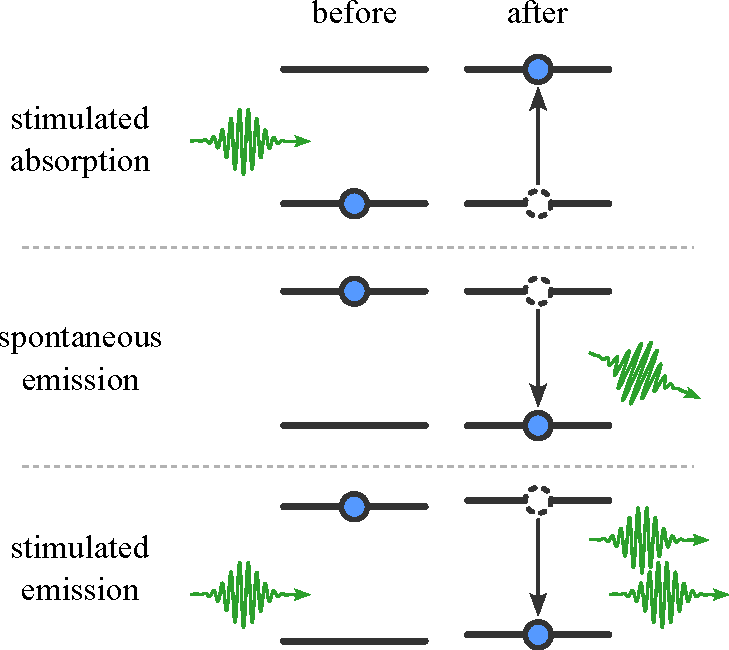
\includegraphics[width=0.55\textwidth]{lesson5/5-3_three_interactions.pdf}
    \caption[Light-matter interactions]{Three fundamental types of light-matter interactions.}
    \label{fig:5-3_light_matter_interaction}
\end{figure}

We can see from Fig.~\ref{fig:5-3_light_matter_interaction} that stimulated emission starts begins with a single photon and finishes with two coherent photons.
This opens up the possibility of amplifying light, which brings us to the ``light amplification'' part of the laser.
Imagine having a large number of atoms in the excited state.
A single photon of light can stimulate the first atom to emit a photon.
Both photons (the initial one and the newly emitted one) can now stimulate further atoms to emit triggering an cascade of emissions and producing a coherent beam of highly intense light. 
However, there is one catch to the above scheme, and that's that not all of the atoms are usually found in the excited state.
When left alone, the atoms are much more likely to be in the ground state.
Getting all of them into an excited state is no easy task.


Let's do some simple accounting to see what happens to our lasing scheme if we do not assume that the atoms start in the excited state.
The three possibilities when a photon is incident on an atom are compiled in the Table~\ref{tab:5-3_three_possibilities}.
\begin{table}[h]
    \centering
    \begin{tabular}{c|c|c}
        Photons in & Atom & Photons out \\
        \hline
        1 & no interaction & 1 \\
        \hline
        1 & ground state & 0 \\
        1 & excited state & 2 \\
    \end{tabular}
    \caption[Stimulated emission accounting]{Number of photons initially and after the process of stimulated emission between a single photon and single atom.}
    \label{tab:5-3_three_possibilities}
\end{table}
The first possibility is the trivial one, the photon does not interact with the atom and nothing happens.
The photon continues travelling past the atom and the atom remains in whatever state it was.
This is represented by the first row of Table~\ref{tab:5-3_three_possibilities}.
The second possibility is that the photons interacts with the atom while it is in the ground state.
The atom absorbs the energy of the photon meaning the number of photons after the process drops to zero, as seen in the second row of Table~\ref{tab:5-3_three_possibilities}.
The last possibility is that the photon interacts with an atom in the excited state, the atom is stimulated to emit a photon of light which is coherent, resulting in two coherent photons after the interaction as seen in the last row of Table~\ref{tab:5-3_three_possibilities}.
We see that the average number of photons is conserved.
We have three photons before the interaction and three photons after the interaction, meaning a single atom is not able to amplify light purely via stimulated emission.

\begin{figure}[t]
    \centering
    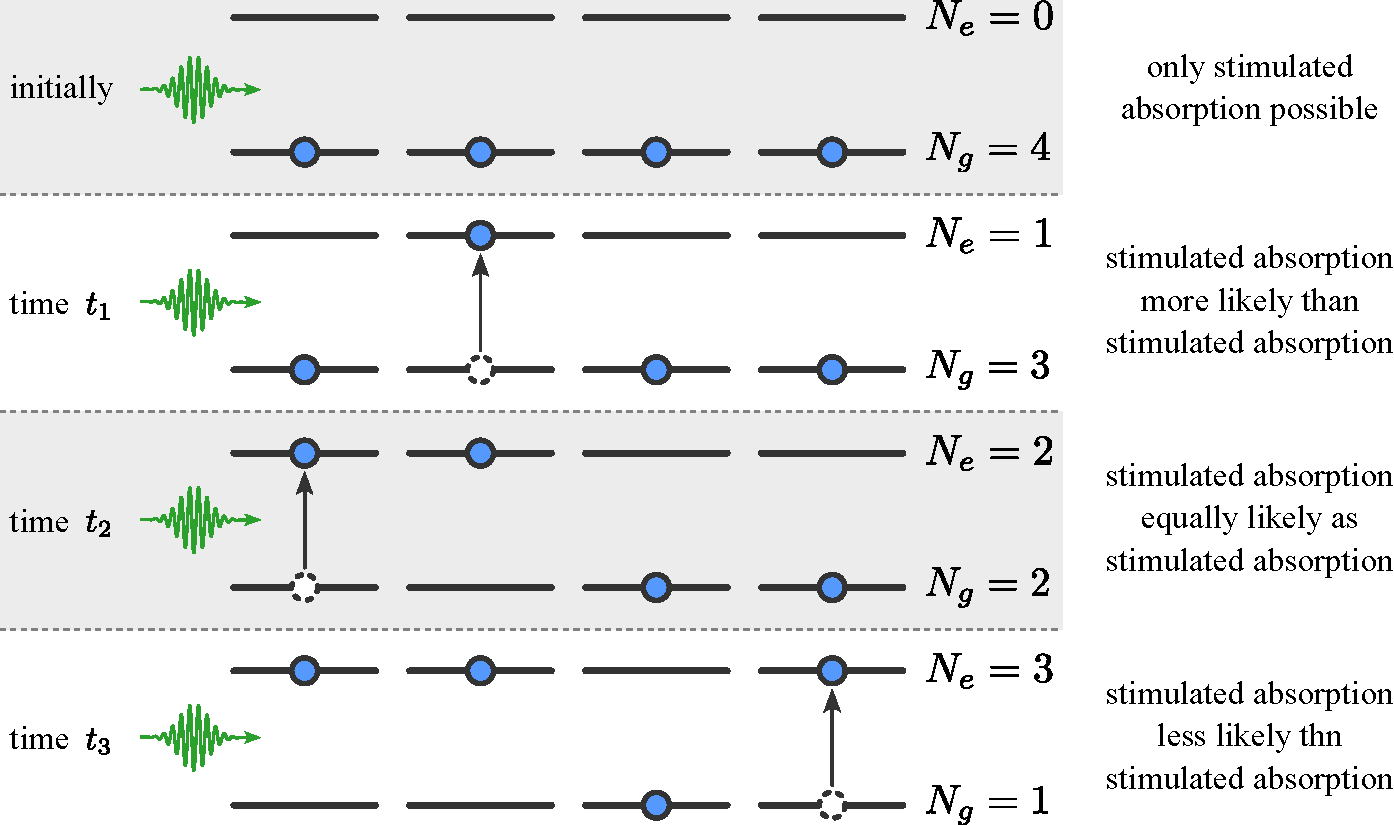
\includegraphics[width=\textwidth]{lesson5/5-3_population_inversion.pdf}
    \caption[Population inversion]{Stimulated emission becomes likely only when most of the atoms are found in the excited state.}
    \label{fig:5-3_population_inversion}
\end{figure}

Therefore it makes sense to consider multiple atoms.
Figure~\ref{fig:5-3_population_inversion} depicts four two level atoms.
Number of atoms in the ground state is denoted by $N_g$, while $N_e$ is the number of excited atoms.
All atoms are initially in the ground state, $N_g=4$.
The only interaction that is possible for an incoming photon is to get absorbed by one of the atoms.
At a later time $t_1$ there is a new incoming photon.
This time $N_e=1$ and $N_g=3$, meaning both stimulated absorption and emission are possible.
However, stimulated absorption is more likely because more atoms are in the ground state.
Let's say that the photon is absorbed by one of the atoms in the ground state.
At time $t_2$, when a new photon is incident on our group of atoms, both stimulated absorption and emission are equally likely since $N_e=N_g=2$.
For the sake of this example, let's say that this photon is absorbed as well, bring the totally tally to $N_e=3$ and $N_g=1$.
Finally, when another photon at time $t_3$ comes along, it has higher chance of stimulating an emission from one of the excited atoms.
This example demonstrates that if we want to achieve light amplification, we require
\begin{equation}
    N_e > N_g.
\end{equation}
This condition is known as \textit{\textbf{population inversion}}.

It seems that we now have a way of producing an intense and highly coherent light.
There is however one final obstacle that needs to be overcome.
We have seen in Fig.~\ref{fig:5-3_population_inversion} that if $N_g > N_e$, then the incoming photon is more likely to be absorbed and contribute to the population of the excited state.
On the other hand, when $N_g < N_e$, then the incoming photon is more likely to stimulate an emission from one of the excited atoms, contributing to the population of the atoms in the ground state.
This means that in the long-time limit, the population of atoms approaches an equal distribution where $N_g = N_e$.
This means that population inversion is not possible to be achieved for an ensemble of two-level atoms.



\section{Lasers II: Population inversion}
\label{sec:5-4_lasers2}

We said in the previous step that in order to create "population inversion", we require a three level atom. So, this is our new atom. It's got three levels and we rename the ground state to E1, the previous excited state was E, but now we're going to call it E2, and then there's another level of higher energy which we are going to call E3.

And, this new introduced level is an unstable level, meaning that whenever we excite the atom to energy E3, then it quickly decays- it doesn't spend much time in this highest level, and this transition between E3 and E1 will be referred to as the "pumping transition".

And this transition between E2 and E1 is our original "lasing transition".

So the goal is to create population inversion by exciting the atom to E2, but without actually affecting the lasing transition, meaning somehow we need to excite the atom to E2 without causing stimulated absorption between E1 and E2. So let's see how to do that. Consider a photon coming in that's tuned to the pumping transition's energy, so its energy is equal to the difference between E3 and E1. What that does it causes stimulated absorption of the ground state atom. It absorbs the energy of the photon and it gets excited to energy level E3. And at the same time, it does not affect the lasing transition at all, so the atom does not get excited from E1 to E2 purely because the photon- the blue photon that caused the stimulated absorption is tuned to the transition between E3 and E1. And as we said, the level E3 is unstable, so it quickly decays to level E2, and then once it's there it can interact with an incoming photon that's of the correct frequency given by the lasing transition, and as we saw what can happen is stimulated emission, and we obtain two photons of the same frequency, traveling in the same direction, and that are both in phase meaning that they are coherent. So this is the cycle. We are irradiating the photon by two light sources. One light source- this black one, is tuned to the lasing transition and it's responsible for causing the stimulated emission, and that's basically our laser light. And there is also this pumping photon coming in that's responsible for exciting the atom to E3 which then quickly decays to E2. So the pumping photon is responsible for creating a population inversion.

%And that's what we said.

This is what we predicted. \rdv{? okay ?}

What we end up with is if we have many such three-level atoms, we end up in the situation where N2- so the number of atoms in the level E2, is larger than the number of atoms in level E1, and if the pumping rate is high enough then all of the atoms that are in the ground state, they are more likely to get pumped into E2 rather than absorbing the incoming black photons and getting excited to level E2.

So, now let's start to build our laser. All of these dots- they represent our three level atoms, and we're going to refer to this as a "gain medium". And a gain medium can be either solid, it can be a gas, or it can be a liquid. So without doing anything, most of the atoms are found in the ground state. Occasionally, some of them get excited and what happens is they decay via spontaneous emission, and they are giving out light in all directions. But, we want to obtain lasing action- we want all of the light to be coherent. So what we do- as we saw, we must create population inversion, and to do that we start pumping the medium represented by these blue arrows, so what that does it excites our atoms first to level E3, then it quickly decays to level E2.

We, in fact, do get some stimulated emission, but still we are getting also some spontaneous emission, but most importantly the photons that we get via stimulated emission- they are escaping our gain medium. What we can do to prevent this is actually build mirrors from both sides. This will increase the number of photons inside the gain medium that will later be part of this cascading process of creating more and more coherent photons. So now we are pumping our gain medium, we've got 100 percent reflective mirrors on both sides, and what happens, in fact, we see lasing action inside the medium. The pumping creates population inversion and then the existing photons that are inside the gain medium stimulate emission on the lasing transition, creating more copies of those photons and again cascading into a lasing action.

So, we created a laser. The only problem is- the light is confined within the gain medium, and somehow we need to get it out. So what we do- we take one of these mirrors and we make it partially reflective, and "partially" here means that it's 99 percent reflective. So what happens, the photons inside the gain medium, they've got some probability to actually escape out and they in fact do, and what we get is a nice, monochromatic, in-phase, traveling-in-the-same-direction light, and this is basically the basic principle of constructing a laser.

And as we said, the output is coherent.

So, we said that we have to pump our three-level atoms in the gain medium at some level, we have to pump it hard enough. So can we get some physical understanding where the threshold is? And for that, we will write down a very simple, a little bit naive model of how our laser works. Let's say that the number of photons in the gain medium is given by small "n", and that's a function of time (t), the number of excited atoms that we care about because they contribute towards the stimulated emission process, is denoted by capital "N", and that's also a function of time (t).

And the rate of change of photons inside the gain medium is given by the difference between some gain process and some loss process. So let's examine what's the gain. Well, the gain depends both, on the number of photons that are already in the gain medium, and on the number of excited atoms. If we don't have any photons, then we cannot cause any stimulated emission. If we don't have any excited atoms, again we don't get any stimulated emission. So we can model the gain term as follows- we've got some "G"- some proportionality constant, which we're just going to call the "gain coefficient", times the number of photons, times the number of excited atoms. Okay, how about the loss? Well as you saw, we lose photons by these photons escaping through the partially reflective mirror. So we can just model it simply as some coefficient "k", which we're going to refer as the "loss coefficient", times the number of photons that are already in the gain medium. If we don't have any photons we have nothing to lose. If we have more photons we are more likely to lose them.

So, this is our model, that the rate of change of the photons inside the gain medium is given by these two terms- gain minus loss. And now comes the crucial bit- this capital N, the number of excited atoms, also depends on time, mainly the stimulated emission that happens decreases the number of excited atoms. And let's say that our pump has the ability to keep the number of excited atoms at some constant level "N-zero" if there is no lasing action, so if there is no stimulated emission happening, this is the number of excited atoms that we have due to the pumping process.

So we can write down an equation for the number of excited atoms simply as: N-zero minus alpha-n, where this "alpha" is the rate of stimulated emission. So substituting everything back into the rate equation for the number of photons, we get the following non-linear dynamical process.

We've got this linear term "n", which depends depends on some combination of these parameters, and then we've got a non-linear term n-squared, which depends on alpha times g. And as you can see, all of our parameters are positive, therefore the graph of this "n-dot" is always a concave parabola. So let's consider one case and plot this graph. On this vertical axis we've got the rate of change, and on the horizontal axis we've got number of photons inside the gain medium. So if n-dot is positive, it means we are increasing the number of photons in the gain medium, and this happens when we have lasing. However, if n-dot is negative, it means that the number of photons is decreasing, there is no lasing, we are simply losing photons, and you can see that if N-zero is such that it is less than k over G, this first linear term in our n-dot equation is negative, and then what happens is our n-dot looks looks like that, and the little arrow on the horizontal axis means that it doesn't matter with how many photons you start in your gain medium. You will eventually lose all of them, meaning the fixed point of this process is at n equals to zero, so no matter how many photons you start, at the end of the day you will always lose your photons. And that's because the coefficient in front of the linear term is negative, but of course we can increase zero, we can just increase the pumping strength such that the coefficient of the linear term is positive, and that's the following scenario. And you see that now, we've got two fixed points- one is still at n equals to zero, but this time this fixed point is unstable, meaning if we have zero photons in the gain medium to start with, of course we will not see any lasing action, and we will remain at n equals zero. However if we just slightly perturb from this situation, if we increase the photon number just slightly, n-dot in that region is positive. It means that we are getting more photons, so we will move along the n-axis until we reach this black circle which is our new stable fixed point. On the other hand, if we start on the right of this fixed point, we start with more photons. We will lose some of them, but we will stop at this finite fixed point, meaning that in this regime when N-zero is larger than the ratio of k and G, we get lazing action.

And we can see that if we plot the number of photons as a function of the pumping strength, which in our model corresponds to capital N-zero.

And in the region where N-zero is less than k over G, our fixed point in terms of n is just zero. Always, we lose all of the photons from our gain medium. But once we increase the pumping strength past this threshold given by k over G, we see that the fixed point for n keeps increasing and is finite. So, in the region where N-zero is less than k over G, we basically have a light bulb. The only source of light that comes from our gain medium is incoherent light. On the other hand, if the pumping is strong enough and N-zero is larger than k over G, we have a laser.

\section{Single photons}
\label{sec:5-5_single_photons}

%Step Five: Single Photons

So we have seen how to generate light in an incoherent state. We have seen how to generate light in the coherence state. And satellite is very useful in classical communication. In particular, it uses- in order to encode zeros and ones in order to code classical bits, it uses large numbers of photons. So on a on a graph, where on the horizontal axis we've got time, and the number of photons on the vertical axis, all of these ones and zeros- these classical bits, here they are represented by some very, very large number. And this has a number of advantages. Number one- it's robust. Even if you lose some of the photons, it's no real big deal. Of course, eventually you will lose most of your photons and your signal will deteriorate, so then what you can do, you can just easily amplify and boost the signal back to its original strength. And also, it allows for quick and deterministic generation. However, such signals are not very useful because we cannot put them in a quantum superposition, and on top of that, because we also cannot entangle such signals between each other, and therefore it's not very useful for quantum communication. Our signals, in order to truly take advantage of quantum mechanics, have to be quantum as well, and for that we have to go beyond lasers and look at single photon sources.

One way of generating single photons is by using attenuated light.

Consider the following scenario- you've got your laser source, and then you've got a bunch of attenuator plates over here represented by these bands. You turn on your laser, it starts at some intensity, but as it passes through the attenuators it loses its intensity until it's so faint that you truly get only single photons represented by these discrete dots over here after the last attenuator. And in principle, this works and we will use this in the next lesson when we look at interference between single photons. However, one big problem of this is that the arrival of these photons is random- it's given by Poissonian statistics, and in order to really be useful in quantum communication, we need something that's not random. So for the purpose of quantum communication, such a scheme is not very valuable and completely not practical. A different scheme that yields single photons is using some kind of heralding mechanism. For example, you can produce two photons, detect one which will also herald the presence of the other, and we already saw such a process in previous lessons, and to remind you it's called "spontaneous parametric down-conversion" (SPDC). So here, you've got some nonlinear crystal, you shine light of certain frequency at the crystal and that produces two photons as your output. Before we used it to produce entangled photons- they were entangled in their polarization. However, here what we can do, we can just detect one of the photons, and if we do then we know that the other photon is also present.

And a couple of advantages of this heralded scheme is that these photons- they travel along a predetermined path, meaning if we detect a photon by our detector, if the detector goes click, then we know exactly where the other photon is traveling. Not only its presence, but also in which direction it's traveling. So it's very easy to couple it to some fiber and then send it off across our quantum network. And on top of that, the rarity of SPDC is actually an advantage. If you recall from previous lessons, this parametric down-conversion, this process, is actually very rare. At best, only we get one pair out of a million photons in state-of-the-art experiments. However here, in this context, that's actually a good thing. It guarantees that if our detector goes click, we've got very high probability that we truly have a single photon and not two or more photons. If SPDC process was more efficient, then it could happen that our detector goes click and here we've got just too many photons, which is not useful for quantum communication.

However, this whole process is still random. Sometimes we get this pair of photons, and even if we get a pair of photons, we have to consider the inefficiencies in the detector. Sometimes it goes click when there isn't a photon. These are known as "dark counts". Sometimes there is a photon and the detector doesn't detect it. So what we are looking for is a single photon, nearly-deterministic source. And such schemes actually do exist.

In particular, you can consider the following structure- again, it's a three-level structure with levels E1, E2, E3, and what you can do is you can excite the atom to level three, which again is short-lived as we saw in our discussion of lasers. It quickly decays to a long-lived level two, and in particular, this level two is long-lived enough such that the pulse that is used to excite to level E3 is finished. So there's a very clear separation between when the exciting pulse is finished and when the atom de-excites from level two to level one, emitting a photon, and it's this photon that is nearly deterministic due to the stability of level two.

Do such materials exist that have this property? In fact, yes, and one example of such a material is known as nitrogen vacancy (NV) centers in diamond. This is a particular material that has many, many nice properties which are very useful in quantum information processing and in quantum communication, and we will come across it again and again. Basically, what it is is- you've got a crystal structure. These green dots- they represent carbon, and you knock one of the carbons out and you replace it with a nitrogen and you knock the other one, and you create a vacancy.

And in particular, these systems have very long coherence times, so we will see them again when we talk about quantum communication protocols, and also quantum memories.


\newpage
\begin{exercises}
\exer{Consider the following quantum state:}
\begin{equation*}
\ket{\psi} = \frac{\sqrt{3}}{2}\ket{0} + \frac{1}{2}\ket{1}
\end{equation*}
\subexer{Find the probability of measuring a zero.}
\subexer{Find the probability of measuring a one.}


\end{exercises}

